
\subsection{Implementado un Event-Handler}

En el contexto de Smart Campus UIS, cada uno de los mensajes enviados por los dispositivos es manejado como un evento. Es decir, cada mensaje recibido debe ser registrado y procesado por los microservicios de administración para lograr un objetivo final. Este procesamiento, recuerda al patrón de diseño \textit{Observer} en el cual se busca el realizar una acción cada vez que el estado, de lo que se está observando, cambia \cite{Shvets2019}.

Siendo así, se estableció el realizar la implementación de un observador el cual se hará responsable de la captura de los mensajes enviados por los dispositivos y establecer el estado del sistema. De esto, como se puede ver en la figura \ref{fig:procesoLooker} se propuso un proceso que debía realizar el observador, apodado \textit{Looker}, a implementar.

\begin{figure}[ht]
    \caption{\\Primera propuesta del proceso a realizar por \textit{Looker}} 
    \centering
    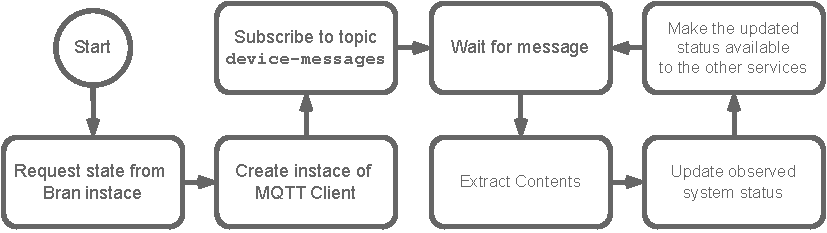
\includegraphics[width=\linewidth]{images/LookerProcess.pdf}
    \label{fig:procesoLooker}
\end{figure} 

Este primer acercamiento, es bastante directo en cuanto a la implementación a realizar. Tras adquirir la definición del estado objetivo, se inicializa un cliente de MQTT, conectado el broker usado por Smart Campus UIS y subscrito al tópico usado por los dispositivos, \texttt{device-messages} \cite{SmartCampusGithub}, este empezaría a procesar los mensajes a medida que estos van llegando. 

Cada mensaje recibido se somete a un conjunto de pasos para actualizar el estado de la aplicación. La figura \ref{fig:LookerProcessUpdateState} describe el proceso que el observador debe realizar con el fin de procesar los mensajes recibidos, dando como resultado, una versión actualizada del estado de la aplicación. 

\begin{figure}[ht]
    \centering
    \caption{\\Proceso realizado por el observador durante el consumo de los mensajes enviados por los dispositivos} 
    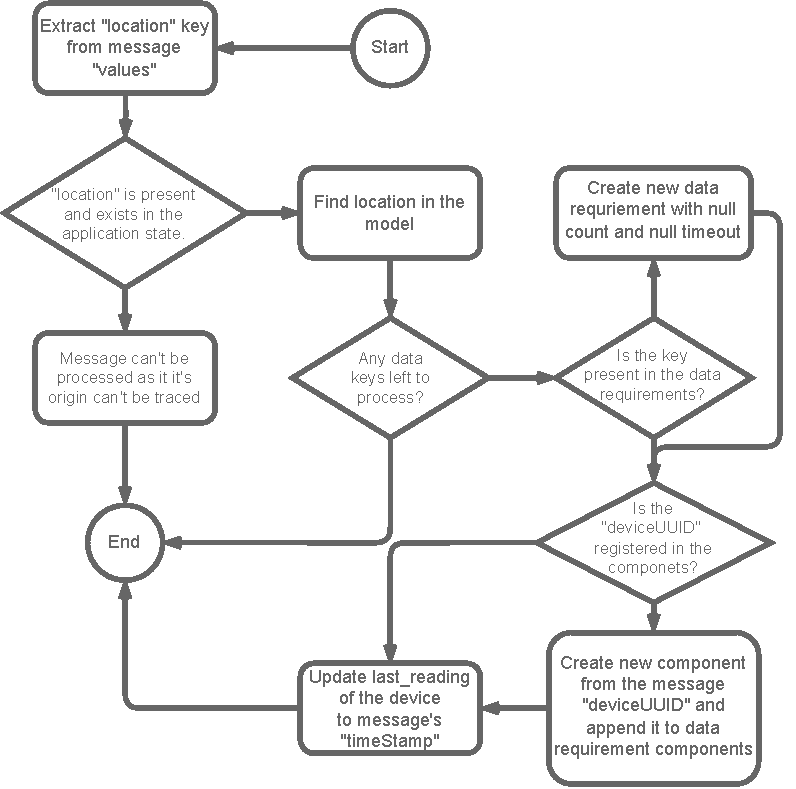
\includegraphics[width=0.70\linewidth]{images/LookerProcessUpdateState.pdf}
    \label{fig:LookerProcessUpdateState}
\end{figure} 

Lo primero a realizar, es ubicarse en el ubicación origen del mensaje. Esto se realiza buscando en las locaciones registradas en la aplicación, usando la llave (Ver figura \ref{fig:jsonSCU}) presente en el mensaje enviado por el dispositivo. En caso que esta, no esté presente, o la locación no haya sido referenciada en la declaración del estado objetivo, el mensaje será descartado. Se debe resaltar que, este puede ser uno de los principales puntos de falla debido a los posibles errores que se puedan presentar al usar nombres diferentes para una locación, sea en los mensajes enviados por problemas en la configuración; o en el momento de la creación del estado de referencia. 

Una vez localizado el origen geográfico del mensaje, se recorrerán los datos reportados por los dispositivos. Estos se cruzarán contra los requerimientos de datos, actualizando los tiempos de los componentes; o registrándolos en caso de que sea el primer mensaje publicado por ellos. Esto se realizará para todas los datos enviados por el dispositivo.
 
